\documentclass{article}
\usepackage[pdftex]{graphicx}
\usepackage{fullpage}

\begin{document}

\title{Modern Physics Laboratory\\
Electron Diffraction}
\author{Josh Diamond and John Cummings}
\date{Fall 2020}
\maketitle


\section{Theory}

The purpose of this experiment is to demonstrate the wave nature
of electrons. A beam of electrons accelerated by a potential of several kilovolts is Bragg
diffracted by a polycrystalline graphite film, and the resulting ring pattern is analyzed to study the
relationship of the electron wavelength to its energy.

\subsection{Electron Wavelength}

A fundamental principle of quantum mechanics is the wave-particle
duality, which states that on the atomic level an object such as
electron, originally thought of as particle, can also exhibit wave
behavior.  Also, light, typically thought of as a wave, can exhibit
particle (photon) behavior.  The wavelength $\lambda$ associated
with a particle of momentum p is given by the relation originally
proposed by deBroglie:

\begin{equation}
\lambda = h/p
\label{eq:debroglie}
\end{equation}

where $p = mv$ is the electron momentum (we assume the electron motion is
non-relativistic) and $h$ is Planck's constant.  The
electron momentum $p$ is directly related to its kinetic energy $K$ by:


\begin{equation}
K = {1 \over 2} mv^2 = {p^2 \over 2m}
\label{eq:ke}
\end{equation}

In this experiment electrons acquire their kinetic energy by being
accelerated (essentially from rest) through a potential difference
$V_a$, where they lose potential energy
$eV_a$ and gain a corresponding amount of kinetic energy,
so that

\begin{equation}
K = eV_a
\label{eq:kev}
\end{equation}

The first experimental observation of the wave behavior of electrons
came in an experiment involving diffraction of electrons by a
crystalline solid---in principle very similar to this one. Such
diffraction is understood to be a wave phenomenon, and observing it
with electrons confirmed their wave aspect.

\subsection{Bragg Diffraction, Bragg's Law}

When a beam of plane electromagnetic waves (such as X rays) of a single
wavelength strikes a crystalline solid, the incident wave interacts
with the charged particles in each atom of the solid, causing them to
emit individual secondary waves which combine to form an outgoing
diffracted beam.  Bragg showed that this process could be described by
a simple physical picture.  One draws sets of equivalent parallel
planes through the atoms of the crystal; each distinct set of planes is
called a ``family'' of planes.  If
the incoming beam makes an angle $\theta$ with the planes in a given
family, the then, the outgoing beam makes the same angle with the
planes---as if the beam were simply {\em reflected} from the plane.
 The outgoing beam is generally rather weak, but when the atoms in
adjacent planes emit waves that are in phase, then these waves combine
constructively to produce an intense outgoing beam, known as a
``Bragg reflection''.  These intense
reflected beams occur when the Bragg's Law is
satisfied, i.e., when 

\begin{equation}
2 d \sin\theta = n\lambda
\label{eq:bragglaw}
\end{equation}

where $n = 1,2,3,\ldots$, $\theta$ is the angle between the incoming beam and a plane in the
family, and $d$ is the perpendicular distance between adjacent planes of
the family.  $n$ is called the order of the Bragg reflection.

As we will discover in this experiment, a beam of electrons exhibits
similar Bragg reflections to those of a beam of electromagnetic waves,
when incident on a crystal.

\section{Preliminary Questions}
\begin{enumerate}
\item Combine Eqs.~\ref{eq:debroglie}--\ref{eq:kev} to obtain an expression for the electron deBroglie
wavelength ${\lambda}$ as a 
function of the accelerating voltage $V_a$.

\item Substitute numerical values for the various quantities and show
that if $\lambda$ is expressed in units of Angstroms (\AA) and $V_a$ is
expressed in volts (V), then it follows that:

\begin{equation}
\lambda(\AA) = {12.26 \over \sqrt{V({\rm V})} }
\end{equation}

NOTE: $1 {\rm \AA} = 10^{-10} {\rm m}$

\item The smallest spacing between the atoms in a metallic copper crystal
is 2.56  \AA. What accelerating voltage is needed
to produce electrons with deBroglie wavelength equal to that spacing?
\end{enumerate}

\section{Equipment}
Teltron electron diffraction tube, filament power supply (AC), high voltage power supply (DC), voltmeter, Vernier calipers

\subsection{Notes on equipment}

The essential interactions of the experiment take place in an evacuated
tube, as shown in Figure~\ref{fig:schematic}. 
\begin{figure}
\begin{centering}
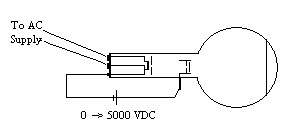
\includegraphics[width=3.0929in,height=1.3543in]{images/ediffraction-img1.png}
\caption{Schematic diagram of electron diffraction tube.}
\label{fig:schematic}
\end{centering}
\end{figure}
Electrons are emitted from a heated filament,
accelerated by potential difference $V_a$.  The beam of
electrons is incident on a graphite film.  The outgoing electrons are
detected by means of the light they produce when striking the
phosphorescent coating of the tube. 

As shown in Fig.~\ref{fig:schematic}, the tube contains four terminals for electrical
connections, two for the AC voltage (6 V) that serves to heat the
filament and two for the DC accelerating voltage $V_a$.
 Note that the two larger receptacles on the base of the tube connect
to AC terminals of the power supply.  The smaller receptacle is to be
connected to the negative DC terminal.  The positive DC voltage
terminal is connected to the plug pointing perpendicular to the tube
axis located near the graphite film.

The graphite film is polycrystalline---composed of large number of
crystallites (very tiny perfect crystals) randomly oriented within the
material.  Referring to Bragg's law (Eq.~\ref{eq:bragglaw}), we note
that for a given order $m$ (say $m$ = 1) and a given $d$ (for a particular
family of planes), there is only one value of the angle ${\theta}$
which satisfies the Bragg condition for a strong reflection.  If our
sample consisted of a single crystal, we would have to rotate it into
position so that the planes would be at the proper angle for the Bragg
reflection.  However, with our polycrystalline sample, there will
always be some crystallites in the proper orientation to give a Bragg
reflection at that angle, as illustrated in Figure 2 below.
\begin{figure}
\begin{centering}
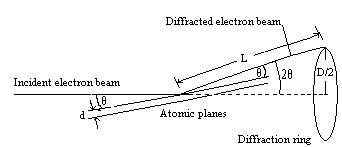
\includegraphics[width=3.5634in,height=1.5311in]{images/ediffraction-img2.png}
\caption{Diffracted electron beam, with ring pattern produced on phosphorescent coating of tube}
\label{fig:rings}
\end{centering}
\end{figure}

The figure shows an upward reflection, but downwards or sideways
reflections will also occur. Considering all these possibilities, it is
easy to see that the reflected electron beams will travel along the
sides of a cone whose vertex lies at the point where the electron beam
is incident on the sample, and with half-angle equal to $2{\theta}$.
 When these beams strike the spherical end of the tube with the
phosphorescent coating, the coating is illuminated in a ring-shaped
pattern.

In this experiment, the angle ${\theta}$ is small enough so that the
small-angle approximations, $\sin\theta \approx \theta$ and $\sin2\theta \approx 2\theta$  hold with sufficient accuracy.  Using
Bragg's law, Eq.~\ref{eq:bragglaw}), we can then relate the measured
ring diameter $D$ to the Bragg angle $\theta$ and hence to the electron
wavelength (see Fig.~\ref{fig:schematic}):

\begin{equation}
{ D/2 \over L } = \sin2\theta \approx 2\theta \approx 2\sin\theta = n\lambda/d
\end{equation}

and hence

\begin{equation}
D \approx {2nL\lambda\over d}     
\end{equation}

Note that for this apparatus, the distance L from the graphite sample to
the phosphorescent screen has the value $L = 13.5 {\rm cm} $.

\section{Procedure }

\begin{centering}
{\bf CAUTION}
\end{centering}

This experiment uses voltages up to 5000 volts DC.
Keep hands away from high voltage power supply
connections.  Ask instructor to check circuit before
turning on power supply.

\begin{enumerate}
\item Turn on the power supply. The DC voltage should be set at zero.
Wait approximately one minute for the AC current to heat the filament
and for the filament temperature to stabilize.  Then turn up the DC
voltage (which is the accelerating voltage $V_a$ for the
electron beam) and set at 4000 volts.  Two circular Bragg diffraction
rings should be visible on the phosphorescent coating of the tube.

NOTE: The room should be darkened so that the rings are more visible.
 Use the lamp provided to assist in taking measurements and recording
data.

\item Point the bar magnet perpendicular to the straight part of tube,
near the middle of the straight section.  How is the Bragg diffraction
ring pattern affected?  Using the right-hand rule, predict the
direction of the magnetic force on the electrons, assuming that they
behave as a beam of particles.  Compare to the observed deflection of
the ring pattern.  Note that in this step, you are observing both
the wave nature and particle nature of the electrons with the same
apparatus.

\item NOTE: For these observations, it is best to view the rings by
looking at the inner surface of the spherical part of the tube \ (where
the phosphorescent coating is located).

Adjust the accelerating voltage $V_a$  gradually up and
then down.  What is the effect on the size of the diffraction rings
when $V_a$ is increased?

\item Set the accelerating voltage at 3000 volts.  Using the Vernier
calipers provided, carefully measure the diameter of each of the two rings.  Repeat these
measurements for four more values of $V_a$ up to a
maximum of 5000 volts, increasing $V_a$ in increments of
500 volts.
\end{enumerate}

\section{Analysis}

\begin{enumerate}
\item Give a qualitative explanation (in words) for the relationship you
observed between the diffraction ring diameter and the accelerating
voltage.  HINT:  the explanation can be based on the deBroglie
hypothesis and a general property of Bragg diffraction.  See the above
equations and accompanying discussion.

\item Based on the theory and the equations discussed for this experiment,
derive an expression for the ring diameter $D$ as a function of the accelerating voltage
$V_a$. This expression should be in the form of a power
law.  What is the theoretically predicted exponent of
$V_a$ in this power law?

\item Plot on logarithmic axes the experimental values of $D$ vs.
$V_a$ for your outer ring data. Does the graph indicate a power law relationship?  Use an appropriate curve
fit to find the exponent of $V_a$ , and compare it to the
theoretical value.  Repeat for the inner ring data.

\item For the outer ring data, calculate the atomic plane separation $d$ for
each value of $V_a$ used. Express your results for d in Angstroms.

HINT: Use your data for $D$ and the theory and equations discussed
previously.  The result of Preliminary Question 2 may be helpful.

(NOTE: It turns out that in this experiment we observe only the
first-order Bragg reflections, so take $n = 1$ for these calculations.)

Find the mean value of d and the uncertainty in the mean.

\item Repeat the calculations of step 4 for the inner ring data.

\item The crystal structure for graphite---our diffracting
material---is hexagonal. The carbon atoms lie in parallel layers and, within each layer, are located at the vertices of regular hexagons.  The separation between adjacent
atoms is 1.42 \AA.  The two families of parallel crystal planes
corresponding to the two diffraction rings observed in this experiment
are shown in Figure~\ref{fig:graphite} below.
\begin{figure}
\begin{centering}
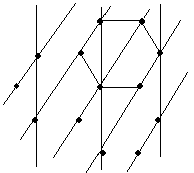
\includegraphics[width=2.0209in,height=1.802in]{images/ediffraction-img3.png} 
\caption{Crystal structure of graphite, showing the two observed families of planes.}
\label{fig:graphite}
\end{centering}
\end{figure}

For each of the two families of planes shown in the figure, use geometry
and trigonometry to calculate a predicted value of $d$ (the perpendicular
distance between adjacent planes).  Compare these values to the
corresponding results for $d$ determined from your measurements, taking
the experimental uncertainty into account.

%\item In Procedure, step 2 it was stated that you observed both the
%particle and wave nature of the electrons.  Explain specifically how
%that was achieved in that step.  Look up Bohr's
%principle of complementarity in a modern physics textbook.  What does
%that principle say?  Was that principle violated by your observations
%in step 2?  Discuss briefly.
\end{enumerate}

\section{Reference}
\begin{itemize}
\item French and Taylor, An Introduction to Quantum Physics, pp. 72-78
\item Thornton and Rex, Modern Physics $3^{\rm rd}$ edition, pp. 171-173
\item Tipler and Llewellyn, Modern Physics $5^{\rm th}$ edition, pp. 185-192
\end{itemize}


\end{document}
